The Airbag Note is designed for investors who want to profit from further growth of \gls{jpm} and still be protected against moderate losses.
At maturity on January 15, 2027, the payoff depends on the final price of \gls{jpm}:
\begin{itemize}
    \item If the stock ends at or above its initial price $S_0$, the investor receives the invested capital plus a share $p$, the participation rate, of the stock's gain.
    \item If the stock ends below $S_0$ but above the airbag level $A$, the investor still receives the full capital.
    \item Only if the stock falls below the airbag level does the payoff drop, in proportion to the stock's performance.
\end{itemize}
The airbag works as a cushion against moderate declines, which makes the note suitable for risk-conscious investors who still want to take part in \gls{jpm}'s upward trend.

\subsection{Payoff}
The payoff at maturity depends on $S_T$, the participation rate $p \in (0, 1)$ and the airbag level $A \in (0, S_0)$.
It is convenient to write it as $N \cdot \varphi_{p,A}(S_T)$, where the payoff factor $\varphi_{p,A}$ scales the initial investment $N$:
\begin{equation}
\label{eq-airbag-replication-phi}
    \text{Payoff}_{p,A}(S_T) = N \cdot \varphi_{p, A}(S_T) =
    N \cdot \begin{cases}
        1 + \frac{p}{S_0} (S_T - S_0), & \text{if } S_0 \leq S_T,\\[6pt]
        1, & \text{if } A \leq S_T < S_0,\\[6pt]
        \frac{S_T}{A}, & \text{if } S_T < A.
    \end{cases}
\end{equation}
The three cases correspond to a gain ($\varphi > 1$), preserved capital ($\varphi = 1$) and a loss ($\varphi < 1$).
Working with $\varphi$ lets us analyse the product independently of the amount invested.
For this product, we set the airbag level to $A = 0.8\,S_0 = 256.33$.
The payoff is shown in Fig.~\ref{fig:airbag-payoff}.

\begin{figure}[H]
    \centering
    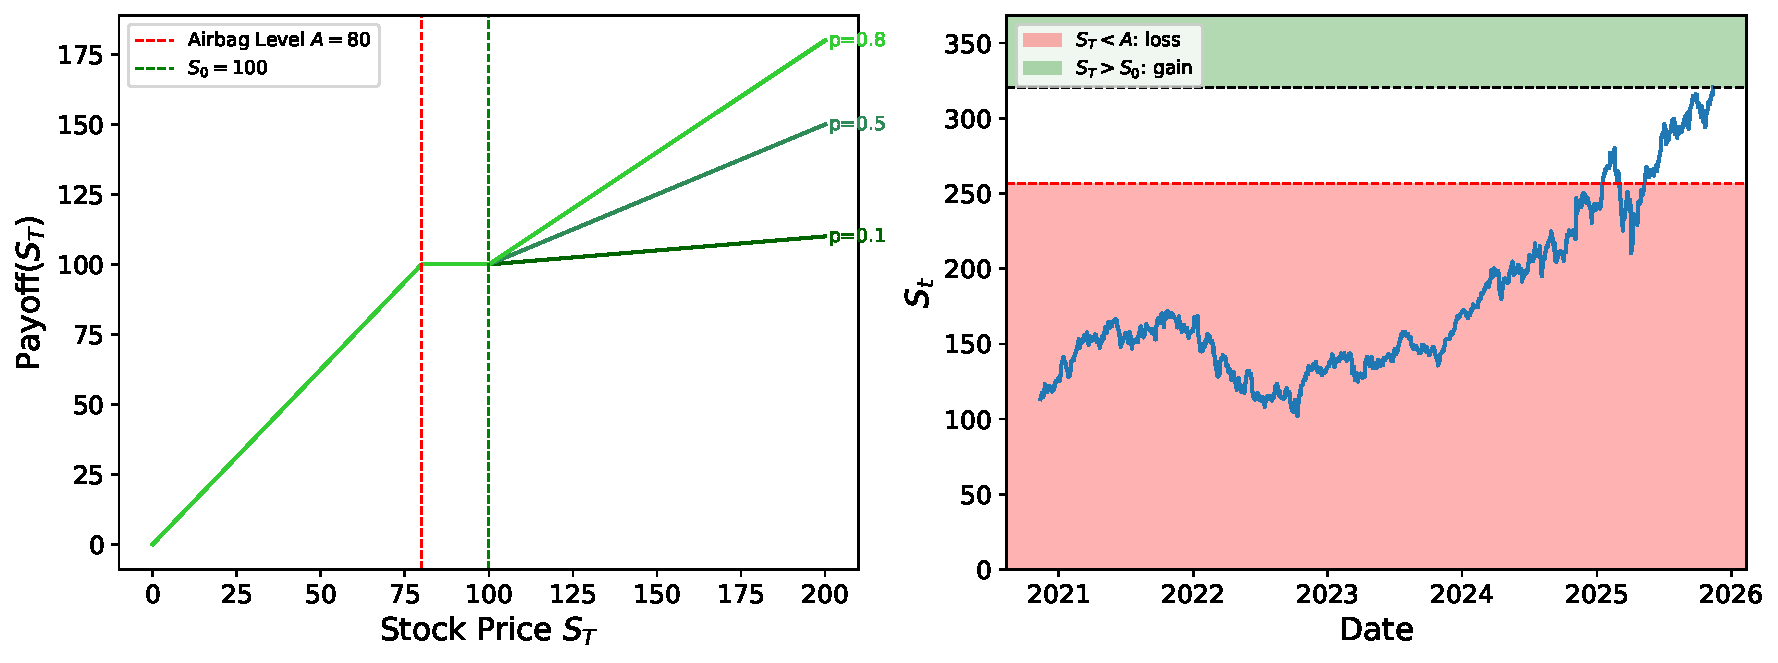
\includegraphics[width=\linewidth]{airbag_payoff.pdf}
    \caption{\textbf{Airbag Payoff.} Left: payoff for $N = 100$, $S_0 = 100$ and $A = 80$ with different participation rates. Right: closing prices of \gls{jpm} over the past five years with the airbag level $A = 256.33$ and the spot price $S_0 = 320.41$. The investor gains above $S_0$ (green), keeps the capital between $A$ and $S_0$ (white) and makes a loss below $A$ (red).}
    \label{fig:airbag-payoff}
\end{figure}

\subsection{Replication}
The payoff \eqref{eq-airbag-replication-phi} can be rewritten as
\[
    \text{Payoff}_{p, A}(S_T)
    = N \left( 1 + \frac{p}{S_0} (S_T - S_0)^+ - \frac{1}{A} (A - S_T)^+\right).
\]
This form shows the replicating portfolio directly: a zero-coupon bond that pays $N$ at maturity, a long position in $\frac{Np}{S_0}$ European calls with strike $S_0$, and a short position in $\frac{N}{A}$ European puts with strike $A$.
Including the issuer's margin $M = mN$ as before, the cost at $t = 0$ must equal the investment:
\begin{align*}
    N &= N \left( e^{-rT} + \frac{p}{S_0} EC(S_0, T) - \frac{1}{A} EP(A, T) + m \right) \\
    \Rightarrow \quad 1 &= e^{-rT} + \frac{p}{S_0} EC(S_0, T) - \frac{1}{A} EP(A, T) + m.
\end{align*}
Since both strikes are fixed, the only free parameters are the margin $m$ and the participation rate $p$.
Solving for $p$ gives a linear function of the margin:
\begin{align}
    p(m)
    = \underbrace{\left( 1 - e^{-rT} + \frac{1}{A} EP(A,T) \right) \frac{S_0}{EC(S_0,T)}}_{\alpha}
    \;+\;
    m \underbrace{\left( - \frac{S_0}{EC(S_0,T)} \right)}_{\beta}.
\end{align}
Neither $S_0 = 320.41$ nor $A = 256.33$ is a quoted strike.
We therefore interpolate the option prices linearly between the two nearest strikes: $EC(320.41, T)$ between the calls at 320 and 330, and $EP(256.33, T)$ between the puts at 250 and 260.
The resulting values are listed in Table~\ref{tab:airbag-parameters}.

\begin{figure}[t]
    \centering
    \begin{minipage}{0.48\textwidth}
        \centering
        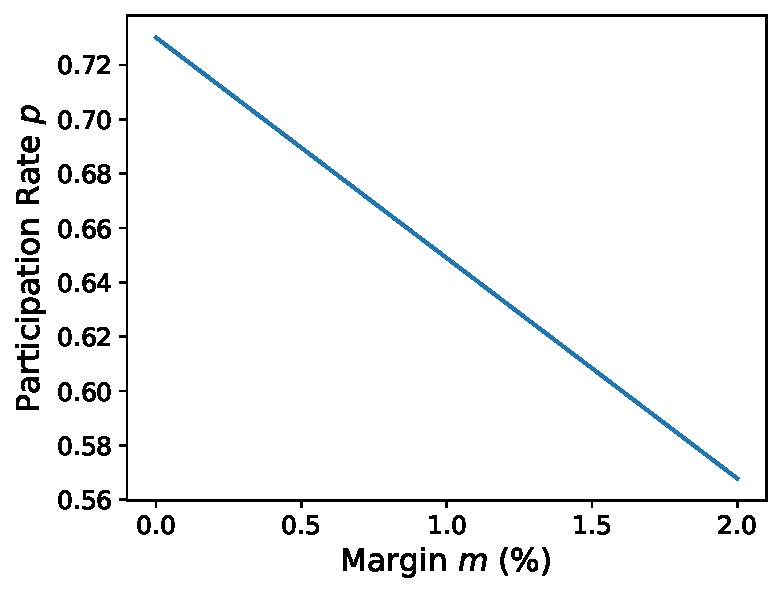
\includegraphics[width=\linewidth]{airbag_participation_vs_margin.pdf}
        \caption{\textbf{Participation vs.\ Margin.} Participation rate $p(m)$ for margins $m$ between $0\%$ and $2\%$.}
        \label{fig:airbag-participation-vs-margin}
    \end{minipage}%
    \hfill
    \begin{minipage}{0.48\textwidth}
        \centering
        \begin{tabular}{ll}
            \hline
            Parameter & Value \\
            \hline
            $r$ & 0.03635 (3.635\%) \\
            $T$ & 1.167 (14 months) \\
            $S_0$ & 320.41 \\
            $A$ & 256.33 \\
            $EC(S_0,T)$ & 39.49 \\
            $EP(A,T)$ & 12.42 \\
            \hline
            $\alpha$ & $\approx 0.730$ \\
            $\beta$ & $\approx -8.11$ \\
            \hline
        \end{tabular}
        \captionof{table}{\textbf{Parameters.} Inputs for the participation rate $p(m)$, where $\alpha$ is the intercept and $\beta$ the slope.}
        \label{tab:airbag-parameters}
    \end{minipage}
\end{figure}

Fig.~\ref{fig:airbag-participation-vs-margin} shows this linear relationship for margins between $0\%$ and $2\%$.
Without a margin, the investor would participate with $p(0) = 0.730$; at $m = 2\%$, the participation falls to $p(0.02) = 0.568$.
As for the \gls{pppn}, we choose $m = 0.5\%$, which gives a participation rate of $p(0.005) \approx 0.690$.

\subsection{Simulation}
We assess the Airbag Note with the same simulated paths as the \gls{pppn} (Sec.~\ref{sec-pppn-simulation}), this time evaluating the payoff factor $\varphi_{p,A}(S_T)$.
Over $10^4$ paths, the note ends with a gain in $76.4\%$ of the cases, preserves the capital in $16.2\%$, and makes a loss in only $7.4\%$.
The expected payoff factor is
\[
    \hat{\mathbb{E}}[\varphi_{p, A}(S_T)] = 1.234 > 1,
\]
which means an expected growth of $23.4\%$ on the initial investment.
Fig.~\ref{fig:jpm-simulation-airbag} shows 100 of the simulated paths together with the airbag level.

\begin{figure}[H]
    \centering
    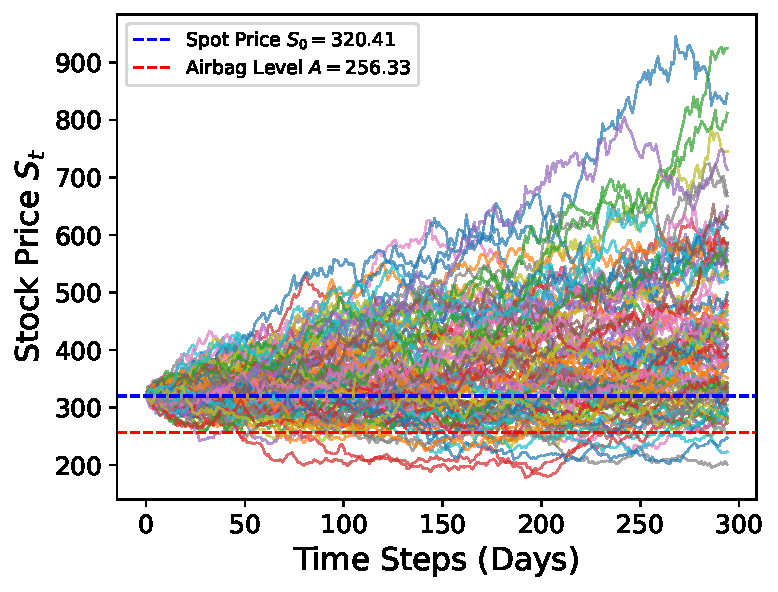
\includegraphics[width=0.5\linewidth]{airbag_simulated_paths.pdf}
    \caption{\textbf{Simulation.} 100 of the $10^4$ simulated paths of \gls{jpm}. The horizontal lines mark the airbag level $A$ and the spot price $S_0$.}
    \label{fig:jpm-simulation-airbag}
\end{figure}
